%-*- coding: utf-8 -*-
\documentclass{beamer}

\usepackage[frenchb]{babel}
\usepackage[T1]{fontenc}
\usepackage[utf8]{inputenc}
\graphicspath{{images/}}

\usetheme{Warsaw}

\title{Projet Vitameal}
\subtitle{Restauration en milieu hospitalier}
\author{Nicolas Symphorien, Sonia Othmani, Jean-Félix Benitez}
\institute{CNAM}
\date{31/03/2017}

\logo{
\includegraphics[height=10mm]{ipst-cnam.png}}
\setbeamertemplate{background canvas}{
\includegraphics[width=\paperwidth,height=\paperheight]{fond_200.png}} % Width pour la largeur, height pour la hauteur de l'image

\begin{document}
\begin{frame}[plain]
  \titlepage
\end{frame}

\begin{frame}
  \frametitle{Sommaire}
  \tableofcontents
\end{frame}

\section{Analyse des exigences}
\begin{frame}[label=analyseDesExigences] %allowframebreaks
\frametitle{Analyse des exigences}
\begin{itemize}
  \item Partie prenantes
  \begin{itemize}
    \item Participantes~: les diététiciens, le service restauration
    \item Concernés~: les médecins, la direction (budget)
    \item Impactées~: les patients
  \end{itemize}
  \item Les besoins
  \begin{itemize}
    \item Les diététiciens renseignent les profils diététiques de chaque patient.
    \item Les diététiciens élaborent les menus.
    \item Le service restauration commande les produits et ingrédients mis en œuvre dans les menus
    \item Le service restauration prépare les menus élaborés.
  \end{itemize}
  \item Les contraintes
  \begin{itemize}
    \item Les médecins doivent pouvoir vérifier / valider les profils diététiques des patients.
    \item La direction fixe un budget maximum par menu.
  \end{itemize}
\end{itemize}
\end{frame}

\subsection{Exigences Fonctionnelles}
\begin{frame}
 \frametitle{Exigences Fonctionnelles}
    \begin{itemize}
    \item Chaque patient a un profil diététique, renseigné par le diététicien
    \item Elaboration automatique des menus, correspondants à un ou plusieurs profils diététiques patients.
    \item À l'issue de l'élaboration des menus, la liste des produits et
      ingrédients (avec leur quantité) est faite afin que le service
      restauration puisse les commander.
    \item La liste des différents menus à réaliser (tickets patients), avec les quantités, est mise à disposition du service restauration pour faciliter l'assemblage du plateau repas.
    \item Ajout de plats.
    \item Chaque plat est décrit avec sa liste d'ingrédients, et la quantité nécessaire à sa réalisation par quantité de poids
    \item Planification des repas par cycles de X semaines
    \end{itemize}
\end{frame}

\section{Planning}
\begin{frame}[label=planning]
\frametitle{Planning}
\begin{figure}[H]
\textbf{G}antt
\label{Gantt}
  \centering
      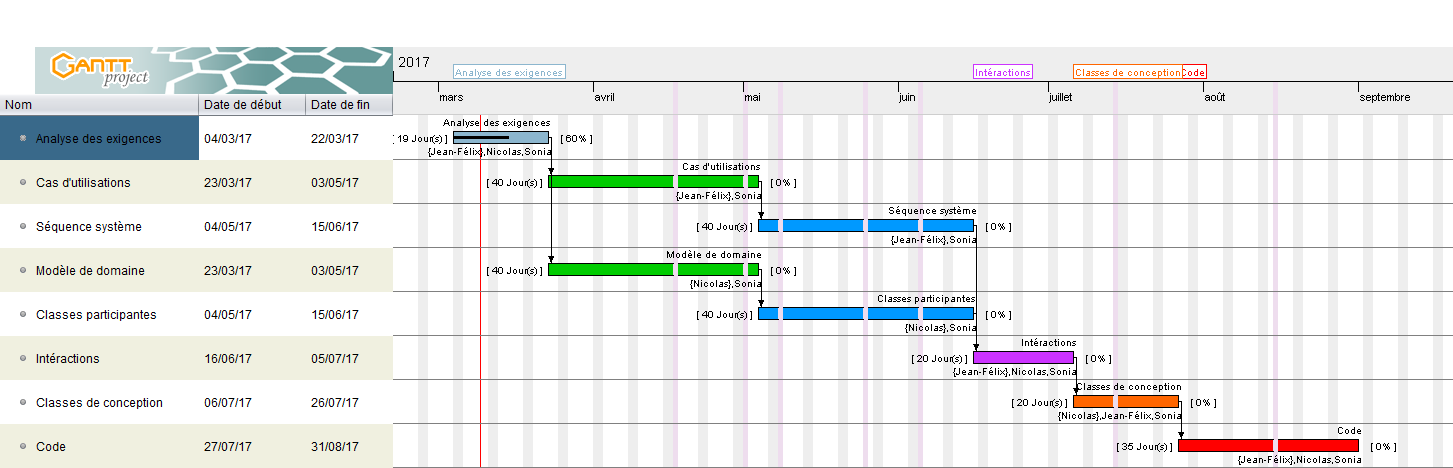
\includegraphics[width=0.95\textwidth]{Vitameal_gantt.png} %
%\caption{Gantt}
\end{figure}

\begin{figure}[H]
\textbf{P}rogram \textbf{E}valuation and \textbf{R}eview \textbf{T}echnique
\label{PERT}
  \centering
      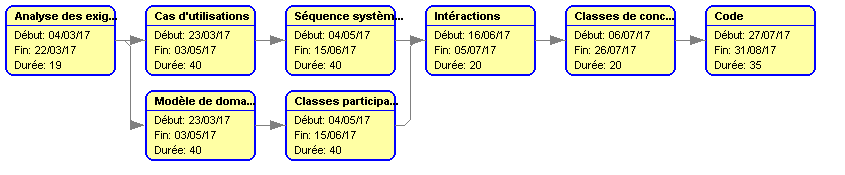
\includegraphics[width=0.95\textwidth]{Vitameal_pert.png} %
%\caption{PERT}
\end{figure}
\end{frame}

\section{Usine logicielle}
\begin{frame}[label=usineLogicielle]
\frametitle{Usine logicielle}
L'usine logicielle de Vitameal répond aux exigences suivantes :
\begin{itemize}
\item respecter les règles de qualités ;
\item avoir une documentation claire et intégrée au projet ;
\item gérer les erreurs et assurer leurs suivies ;
\item versionner le code source et la documentation ;
\item avoir un espace commun accessible à distance ;
\item gérer un espace de livraison générant des indicateurs de santé sur le projet ;
\item avoir un outil de conception UML couvrant la méthode minimal UML;
\item gérer la planification du projet.
\end{itemize}
\end{frame}

\subsection{Documentation}
\begin{frame}[label=documentation]
  \frametitle{Usine logicielle - Documentation}
  \begin{itemize}
  \item utilisation de la syntaxe \textbf{markdown};
  \item intégration à \textbf{GitHub};
  \item usage de \textbf{LaTex} pour les livrables
\end{itemize}
\end{frame}

\subsection{Poste de développement}
\begin{frame}[label=posteDeveloppement]
  \frametitle{Usine logicielle - Poste de Développement}
  \begin{itemize}
  \item \textbf{Eclipse} comme IDE pour écrire/éditer le code de l'application ;
  \item \textbf{Maven} comme constructeur du projet (gestion des dépendances, automatisation de la construction)
  \item \textbf{JUnit} pour écrire les tests unitaires de l'application et Coderturapour analyser la couverture du projet par ces tests ;
  \item \textbf{Git} pour versionnerles sources du projet ;
  \item \textbf{StarUML} pour modéliser selon le standard UML le projet ;
  \item \textbf{GanttProject} pour planifier le projet avec un diagramme de Gantt ;
  \item \textbf{TEXMaker} pour éditer les fichiers «.tex» avec un comportement proche des WYSIWYG (optionnel).
\end{itemize}  
\end{frame}

\subsection{Espace d'intégration continue}
\begin{frame}[label=integrationContinue]
  \frametitle{Usine logicielle - Espace d’intégration continue}
  \begin{itemize}
  \item \textbf{GitHub} comme gestionnaire à distance du repositorie \textbf{Git} principal, comme tracker de bug et comme affichage visuel des taches à faire ;
  \item \textbf{Jenkins} comme serveur d'intégration continue ;
  \item \textbf{SonarQube} comme analyseur de qualité du code.
  \end{itemize}
\end{frame}

\subsection{Schéma de fonctionnement}
\begin{frame}[label=schemaFonctionnement]
  \frametitle{Usine logicielle - Schéma de fonctionnement}
\begin{figure}[H]
\label{schema}
  \centering
      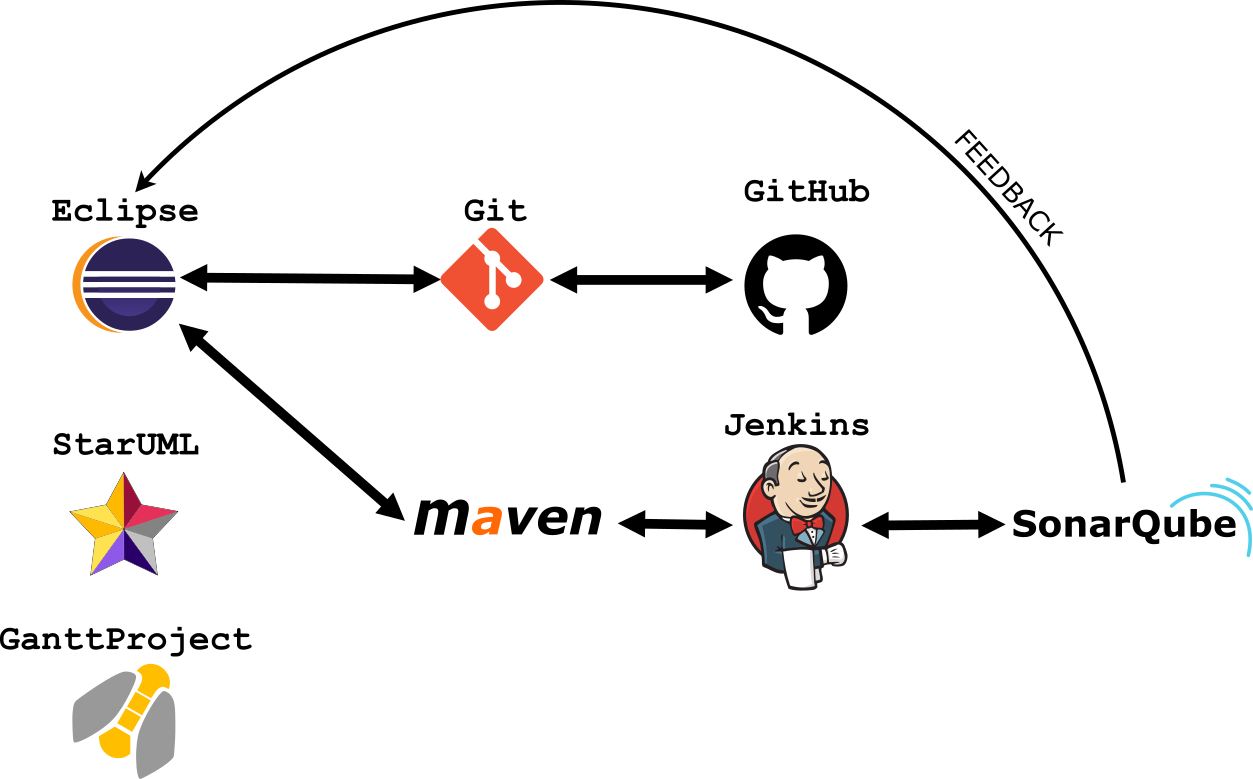
\includegraphics[width=1.0\textwidth]{usine_vitameal.png} %
%\caption{Schéma}
\end{figure}
\end{frame}

\end{document}
